\documentclass[12pt,a4paper]{article}

% =========================
% Temel paket yüklemeleri
% =========================
\usepackage[utf8]{inputenc}
\usepackage[T1]{fontenc}
\usepackage[english]{babel}

% Sayfa yapısı ve kenar boşlukları
\usepackage[margin=2.5cm]{geometry}

% Satır aralığını 1.5 yapıyorum
\usepackage{setspace}
\onehalfspacing

% Matematik ortamları için gerekli paketler
\usepackage{amsmath, amssymb}

% Tablo paketleri
\usepackage{booktabs}
\usepackage{longtable}
\usepackage{array}
\usepackage{multicol}

% Görselleri kullanmak için
\usepackage{graphicx}
\usepackage{float}
\usepackage{caption}

% Linkleri düzenlemek için
\usepackage[hidelinks]{hyperref}
\usepackage[nameinlink,noabbrev]{cleveref}

% Algoritma paketleri
\usepackage{algorithm}
\usepackage{algpseudocode}

% =========================
% Renk tanımları
% =========================
\usepackage{xcolor}
\definecolor{richmaroonxd}{RGB}{186, 52, 90}

% =========================
% Algoritma anahtar kelimelerinin renk ve yazım stilini ayarlıyorum
% =========================
\algrenewcommand\algorithmicprocedure{\noindent\textbf{\textcolor{richmaroonxd}{Procedure}}}
\algrenewcommand\algorithmicwhile{\noindent\textbf{\textcolor{richmaroonxd}{While}}}
\algrenewcommand\algorithmicfor{\noindent\textbf{\textcolor{richmaroonxd}{For}}}
\algrenewcommand\algorithmicforall{\noindent\textbf{\textcolor{richmaroonxd}{For all}}}
\algrenewcommand\algorithmicif{\noindent\textbf{\textcolor{richmaroonxd}{If}}}
\algrenewcommand\algorithmicelse{\noindent\textbf{\textcolor{richmaroonxd}{Else}}}
\algrenewcommand\algorithmicreturn{\noindent\textbf{\textcolor{richmaroonxd}{Return}}}
\algrenewcommand\algorithmicend{\noindent\textbf{\textcolor{richmaroonxd}{End}}}

% Algoritma input-output başlıkları
\algnewcommand\algorithmicinput{\noindent\textbf{\textcolor{richmaroonxd}{Input:}}}
\algnewcommand\Input{\item[\algorithmicinput]}
\algnewcommand\algorithmicoutput{\noindent\textbf{\textcolor{richmaroonxd}{Output:}}}
\algnewcommand\Output{\item[\algorithmicoutput]}

% Fonksiyon isimleri için ufak bir kolaylık
\newcommand{\Func}[1]{\textcolor{richmaroonxd}{#1}}
\usepackage{listings}
\usepackage{xcolor}

% Atom One Light renkleri
\definecolor{atom-bg}{HTML}{FAFAFA}
\definecolor{atom-blue}{HTML}{007ACC}
\definecolor{atom-purple}{HTML}{AF00DB}
\definecolor{atom-green}{HTML}{098658}
\definecolor{atom-gray}{HTML}{6A6A6A}
\definecolor{atom-orange}{HTML}{D16969}

\lstdefinestyle{atomone}{
    backgroundcolor=\color{atom-bg},
    basicstyle=\ttfamily\small,
    keywordstyle=\color{atom-blue}\bfseries,
    stringstyle=\color{atom-green},
    commentstyle=\color{atom-gray}\itshape,
    numberstyle=\tiny\color{atom-gray},
    numbers=left,
    stepnumber=1,
    numbersep=10pt,
    frame=single,
    rulecolor=\color{atom-gray},
    tabsize=4,
    showstringspaces=false,
    breaklines=true,
    emph={
        True, False, None,
        int, float, str, list, dict, set, tuple,
        range, len, print, return
    },
    emphstyle=\color{atom-purple}\bfseries,
    moredelim=**[is][\color{atom-orange}]{@}{@}  % özel vurgular için
}

% Kolay kullanım komutu
\newcommand{\pythoncode}[2]{
\begin{lstlisting}[style=atomone,caption={#1}]
#2
\end{lstlisting}
}
\usepackage{tikz}
\usepackage[table]{xcolor}
\usepackage{pgfplots}
\pgfplotsset{compat=1.18}

% =========================
% Bölüm numaralandırma stilini ayarlıyorum
% =========================
\renewcommand{\thesection}{\arabic{section}}
\renewcommand{\thesubsection}{\arabic{section}.\arabic{subsection}}

% =========================
% Başlık bilgileri
% =========================
\title{\noindent\textbf{Solving the U-shaped Assembly Line Balancing Problem Type-II\\Using a Genetic Algorithm}}

\author{
Firuze İpek Yıldırım \quad 2220469028 \\
Mustafa Alp Ulaş \quad 2210469034 \\
Beril Yıldız \quad 2230469107 \\
Pınar Ece Pank \quad 2240469085 \\
Tarık Buğra Birinci \quad 2210469046 \\[6pt]
\textit{Department of Industrial Engineering, Hacettepe University}
}

\date{Project Final Report\\December 2025}

% =========================
% DOKÜMAN BAŞLANGICI
% =========================
\begin{document}


% KAPAK SAYFASI

\begin{titlepage}
    \centering
    \vspace*{2cm}

    {\LARGE \noindent\textbf{Solving the U-Shaped Assembly Line Balancing Problem Type-II \\[2mm]
    Using a Genetic Algorithm}} \par

    \vspace{1.4cm}

    {\large \noindent\textbf{Project Final Report}} \\[0.4cm]
    {\large EMU427 -- Heuristic Methods for Optimization} \\[0.3cm]
    {\large Department of Industrial Engineering \\ Hacettepe University}

    \vspace{2cm}

    {\large \noindent\textbf{Students}} \\[0.5cm]

    \begin{center}
        \begin{tabular}{l r}
            Firuze İpek Yıldırım & 2220469028 \\
            Mustafa Alp Ulaş     & 2210469034 \\
            Beril Yıldız         & 2230469107 \\
            Pınar Ece Pank       & 2240469085 \\
            Tarık Buğra Birinci  & 2210469046 \\
        \end{tabular}
    \end{center}

    \vspace{1.6cm}

    {\large \noindent\textbf{Instructor:} Prof. Çağrı Koç}

    \vfill
    {\large December 2025 \\ Ankara, Türkiye}
\end{titlepage}


% İÇİNDEKİLER

\tableofcontents
\newpage


% INTRODUCTION

\newpage
\section{Introduction}
% Bu bölümde: U-shaped assembly line kavramı, literatür özeti,
%%%%%%%%%%% !!!!!!!!!!!!!!documentten copy paste yap ipek
% UALBP-II’nin neden önemli olduğu ve GA seçme motivasyonumuz anlatılacak


Assembly line balancing is a fundamental optimization problem in industrial engineering. It aims to distribute tasks across workstations by trying to maximize productivity and minimize idle time. The Assembly Line Balancing Problem (ALBP) is classified as NP-hard, so as the size of the problem grows, methods for obtaining exact solutions become rapidly impractical \cite{becker_scholl_2006_generalized_survey}. As a result, heuristic and metaheuristic approaches have been developed and adapted to obtain high-quality results with reasonable computational effort.
U-shaped assembly lines have significant popularity for being an effective alternative to traditional straight lines in production. They allow workers to work two sides of the line, so it reduces distance and eases multi-tasking.\cite{miltenburg_2001} shows that U-lines can lead to higher productivity and adaptation in changing demand. Type-2 assembly line balancing can be preferred when the number of workstations is fixed. So the first objective is minimizing the cycle time, and it is also suitable for facilities that cannot change their physical line structure, especially with large-sized products\cite{boysen_fliedner_scholl_2007}.
Since the possibilities of assembly line problems get exponentially larger because of their combinatorial structure and growing search area, deterministic optimization approaches remain limited and become computationally infeasible for medium to large scale problems. As a consequence, Genetic Algorithms (GAs) have become an alternative because of their stochastic search methods. In our project, numerous studies we researched mostly highlight that GAs can generate well-performing solutions without the problem needing to be convex or linear as in classical LP problems, so this makes them appropriate for NP-hard manufacturing problems. The essential consideration for U-shaped assembly lines is that the encoding part has to represent bidirectional task assignments and preserve precedence relationships in the evolutionary process.
This project aims to develop and analyze a GA-based approach specifically for Type-2 U-shaped balancing. Even though various metaheuristic approaches are used in classical assembly line balancing problems and show very strong performance in different combinations of the classical assembly line problem, there are a limited number of studies that specifically work on the performance of these algorithms and their applicability for U-shaped Type-2 line balancing. There is a limited number of encoding schemes that represent forward and back task assignments and preserve precedence constraints, while effectively minimizing cycle time in a fixed number of workstations specifically for this problem.

% PROBLEM FORMULATION

\newpage
\section{Problem Formulation - Detailed Problem Description (UALBP-2)}

\par
\subsection{Introduction to Assembly Line Balancing}
Assembly line balancing (ALB) refers to assigning a set of assembly tasks to an ordered
sequence of workstations such that all precedence constraints are satisfied and an efficiency
criterion is optimized. Each task has a processing time, and some tasks must be completed
before others (precedence relations). In straight-line assembly systems, workstations are
arranged linearly, and a task can only be assigned after all of its predecessors are allocated
to earlier stations.

Two classical forms of ALB exist: SALBP-1, which minimizes the number of stations
for a given cycle time, and SALBP-2, which minimizes the cycle time for a given number of
stations~~\cite{scholl_becker_2006,talbot_patterson_gehrlein_1986}. Both are NP-hard combinatorial problems~\cite{garey_johnson_1979}.

\par
\subsection{Characteristics of U-Shaped Assembly Lines}
A U-shaped assembly line is configured such that the beginning and end of the task sequence
are physically adjacent. In this layout, a worker can operate on both sides of the U, giving
access to tasks from the front (forward direction) or the back (reverse direction) of the
precedence graph.

The critical implication is that a task $j$ becomes eligible for assignment if:
\begin{itemize}
\item all its predecessors have been assigned (as in a straight line), or
\item all its successors have been assigned (a U-line specific rule)~\cite{miltenburg_2001,urban_1998}.
\end{itemize}
This relaxation effectively doubles assignment opportunities, allowing U-lines to achieve
better load balancing compared to straight lines. Numerous studies report that U-shaped
lines often require fewer stations and achieve higher efficiency for the same task set~\cite{miltenburg_2001}.

\par
\subsection{UALBP-2 Definition}
UALBP-2 (Type-II U-shaped Assembly Line Balancing Problem) seeks to minimize the
cycle time $c$ for a given number of stations $m$~\cite{scholl_klein_1999}. The input consists of:
\begin{enumerate}
\item a set of $n$ tasks with processing times $t_i$,
\item a precedence graph represented as a DAG,
\item a fixed number of stations $m$.
\end{enumerate}

The output is an assignment of tasks to stations ensuring U-shaped precedence feasibility
while minimizing:
\[
c = \max_{j=1,\ldots,m}\left(\sum_{i\in S_j} t_i\right),
\]
where $S_j$ denotes the set of tasks assigned to station $j$.

\par
\subsection{Assumptions and Constraints}
We consider the standard ``Simple UALBP-II'' variant~\cite{baybars_1986}, which includes the following assumptions:
\begin{itemize}
\item Single-model production: Only one product type is assembled.
\item Deterministic task times: Processing times $t_i$ are fixed and known.
\item Single-sided work: Each worker operates on the inner side of the U.
\item Paced line: The assembly line advances synchronously every cycle time $c$.
\item One worker per station: Each station executes its assigned tasks alone or as a unit.
\item U-shaped precedence feasibility: A task $i$ can be assigned if all predecessors or all
successors satisfy the station-order requirement.
\item Fixed number of stations: $m$ is given and constant.
\end{itemize}

Under these assumptions, UALBP-2 becomes a partitioning problem: partition $n$ tasks
into $m$ ordered groups while minimizing the maximum station load.

\par
\subsection{Computational Complexity}
UALBP-2 is computationally challenging. Even SALBP-2 is NP-hard because it generalizes
bin packing and partition problems with precedence restrictions~\cite{garey_johnson_1979}. UALBP-2 expands the
search space due to bidirectional task eligibility.

Exact algorithms such as branch-and-bound or dynamic programming solve only small
instances~\cite{scholl_klein_1999}. Procedures like ULINO~\cite{scholl_klein_1999} find optimal solutions but exhibit drastic increases
in computation time as $n$ grows. Due to this difficulty and the scarcity of exact solutions
for larger problem sizes, heuristic and metaheuristic methods such as genetic algorithms are
widely recommended.

\par
\subsection{Importance of Solving UALBP-2}
A high-quality U-line balance directly improves production efficiency by reducing idle time
and eliminating bottlenecks. Solving UALBP-2 provides actionable insights for:
\begin{itemize}
\item redesigning assembly processes,
\item increasing output without additional stations,
\item exploiting U-shaped flexibility for smoother workflow.
\end{itemize}
UALBP-2 is therefore a practically significant optimization problem in manufacturing
planning.

\par
\subsection{MILP Formulation for UALBP-2}
We adopt a simplified mixed-integer linear programming (MILP) model inspired by formulations in~\cite{aase_suresh_2003}. The objective is to assign tasks to $m$ stations while satisfying U-shaped
precedence and minimizing cycle time.

% GENETIC ALGORITHM

\newpage
\section{Description of the Genetic Algorithm}
This section presents the metaheuristic approach chosen to solve the U-shaped Assembly Line Balancing Problem Type 2 (UALBP-2): the Genetic Algorithm (GA). Genetic Algorithm is an evolutionary optimization method that takes its inspiration from the concepts of natural selection and genetics. It is particularly suitable for problems in the field of combinatorial optimization where the search space is enormous and discrete.
\newline
The principal concept behind this algorithm is to have a population of candidate solutions (individuals) instead of just one solution. An iterative process, which is similar to evolution, undergoes selection, crossover (recombination), and mutation operations. This, in turn, helps the search to not only simultaneously explore different regions of the solution space but also to realize the benefits of good-quality partial solutions. In the UALBP-2 case, the algorithm works on producing a sequence of tasks (permutation), which is then decoded to find out the minimum feasible cycle time for a certain number of stations ($m$).

\par
\subsection{The Algorithm}
%pseudocode ve gerekirse python code chunk eklenecek
The framework of our Genetic Algorithm is outlined in \cref{alg:ga_ualbp2}.
The core component of the algorithm is the representation of the problem. We use a permutation-based representation, where an individual is a topological sort of the tasks.
The algorithm begins by initializing a random population of feasible task sequences. In every generation, the fitness of each individual is evaluated. Since we are solving UALBP-2 (minimizing cycle time $c$ for fixed $m$), the evaluation function involves a sub-procedure that calculates the minimum possible cycle time for a given sequence.
To generate new offspring, we employ Tournament Selection to choose parents. These parents undergo POX (Precedence Operation Crossover) to produce a child that inherits structural characteristics from both parents. To prevent premature convergence, Swap Mutation is applied with a low probability. Finally, because random genetic operations may violate precedence constraints, a Repair Mechanism is applied to ensure the child remains a valid topological sort.


\begin{algorithm}
\caption{Genetic Algorithm for UALBP-2}
\label{alg:ga_ualbp2}
\begin{algorithmic}[1] % [1] satır numaralarını açar
    \Require Task times, Precedence constraints, Number of stations ($m$), Parameters ($PopSize, MaxGen, P_c, P_m$)
    \Ensure Best Found Permutation and Cycle Time
    
    \State $P \gets \Call{InitializePopulation}{PopSize}$
    \State $BestSol \gets \emptyset$
    
    \For{$gen \gets 1 \noindent\textbf{ to } MaxGen$}
        \ForAll{individual $I \in P$}
            \State $Fitness(I) \gets \Call{EvaluateCycleTime}{I, m}$
        \EndFor
        
        \State $P_{new} \gets \emptyset$
        
        \While{$|P_{new}| < PopSize$}
            \State $Parent1, Parent2 \gets \Call{TournamentSelection}{P, k=2}$
            
            \If{$\Call{random}{} < P_c$}
                \State $Child \gets \Call{POXCrossover}{Parent1, Parent2}$
            \Else
                \State $Child \gets Parent1$
            \EndIf
            
            \If{$\Call{random}{} < P_m$}
                \State $Child \gets \Call{SwapMutation}{Child}$
            \EndIf
            
            \State $Child \gets \Call{RepairToTopological}{Child}$
            \State Add $Child$ to $P_{new}$
        \EndWhile
        
        \State $P \gets P_{new}$
        \State Update $BestSol$
    \EndFor
    
    \State \Return $BestSol$
\end{algorithmic}
\end{algorithm}



\par
\subsection{Implementation}

The \cref{alg:ga_ualbp2} has been developed using the programming language Python due to its excellent high-level data structure handling ability.


\par
\subsubsection{Constructive Heuristic}

When tackling the Type-2 U-Shaped Assembly Line Balancing Problem (UALBP-2), where the aim is to reduce the cycle time for a predetermined number of stations, a major difficulty is that of making the sequence feasible. One of the solutions proposed is to implement topological sorting-based constructive heuristic within the Genetic Algorithm, which draws upon the dependency graph to produce a precedence-feasible list of tasks. This topological ordering not only guides the decoding phase with its precedence constraints but also facilitates the search for the best cycle time by allowing task assignment at either end of the stations.



\subsubsection{Chromosome Representation}
The first alternative became the use of permutation chromosomes where each individual is a series of all n tasks. The order of the genes from left to right indicates the priority that will be applied in the decoding process. This encoding has become the most popular one in assembly-line balancing because it allows the genetic operators to perform the whole task order manipulation without resulting in a non-valid permutation.\cite{GhoshGagne2011}.
Nevertheless, a chromosome in UALBP-2 does not associate with the station assignment directly like in straight-line SALBP-2. On the contrary, the permutation gives an ordered list that the U-line decoding algorithm uses to create a feasible solution. The reason is that U-shaped lines allow the assignments to be done in both directions, thus the decoding phase evaluates the permutation in a manner that shows this unique bidirectional feasibility.\cite{GhoshGagne2011}. 


\subsubsection{U-Shaped Decoding}

Given a task permutation, the decoding procedure assigns tasks to stations progressively from station $1$ to station $m$. At each station, task eligibility is determined by the U-line two-way working rule: a task $j$ is \emph{eligible} if either all predecessors of $j$ have already been assigned or all successors of $j$ have already been assigned \cite{KaraIslierAtasagun2010}. This rule reflects the fact that, in a U-shaped layout, tasks can be performed from both the forward and the backward directions.

Among the currently eligible tasks, those appearing earliest in the chromosome are considered first and are assigned to the current station as long as the cumulative station load does not exceed the current cycle-time estimate. A station is deemed \emph{closed} when no additional eligible task can be inserted without violating the cycle time, after which the decoding continues with the next station.

To evaluate a permutation efficiently, the decoding method incorporates a binary search to determine the smallest cycle time that yields a feasible assignment for the given permutation. This avoids exhaustive trial of cycle-time values and enables fast fitness evaluation \cite{scholl_klein_1999}.

A task $j$ is eligible if
\[
\mathrm{Pred}(j) \subseteq A \quad \text{or} \quad \mathrm{Succ}(j) \subseteq A,
\]
where $A$ is the set of already assigned tasks, and $\mathrm{Pred}(j)$ and $\mathrm{Succ}(j)$ denote the predecessor and successor sets of task $j$, respectively.





\subsubsection{Fitness Function}

Taking into consideration that UALBP-2 is a Type-II problem, the aim is to minimize the cycle time $c$ while the number of stations $m$ is given. The cycle time is determined when a feasible assignment appears by decoding, and it is written as follows:
\begin{equation}
c = \max_{k=1,\dots,m} \sum_{j \in S_k} t_j ,
\label{eq:cycle_time}
\end{equation}
where $S_k$ is the set of tasks assigned to station $k$, and $t_j$ is the processing time of task $j$.

The fitness value is associated with the maximization structure of genetic algorithms; therefore, it is defined as:
\begin{equation}
\mathrm{Fitness} = \frac{1}{c}.
\label{eq:fitness}
\end{equation}

Therefore, solutions with smaller cycle times are awarded higher fitness values. On the other hand, if a permutation does not lead to any feasible assignment for any cycle time (i.e., decoding fails), then its fitness is set to $0$, penalizing such individuals as infeasible. This fitness structure, adopted from the literature, is widely used because it yields positive values, clearly differentiates solution quality, and supports stable convergence behavior \cite{ErelSarin1998}.



\subsubsection{Parent Selection: Tournament Selection ($k = 2$)}
The selection of parents is done by using the tournament selection method of size 2.This has been found efficient for combinatorial optimization problems where the fitness landscape includes many plateaus. The strategy of selection by tournaments is regarded as highly effective for combinatorial optimization problems that have tough fitness landscapes with many plateaus. Tournament selection not only preserves genetic diversity but also avoids a common problem seen in roulette-wheel selection, which is the sensitivity to scaling.
\cite{BlickleThiele1996}




\subsubsection{Crossover Operator: Precedence-Preserving Order Crossover (POX-like)}
When chromosomes represent permutations, standard crossover operators (e.g., one-point or two-point crossover) may easily introduce infeasibility and duplicated tasks. Therefore, the \emph{Precedence-Preserving Order Crossover (POX)} operator is employed \cite{ParkKimLee2003}.

The POX operator proceeds as follows:
\begin{enumerate}
    \item A random subset of tasks is selected.
    \item The offspring chromosome is initialized as an empty sequence.
    \item The selected tasks are copied from Parent~1 to the offspring, preserving their original order.
    \item The remaining tasks are filled according to Parent~2's order, skipping tasks that have already been placed.
\end{enumerate}

This procedure preserves major subsequences from both parents and typically reduces the need for extensive repair operations. POX is particularly suitable for UALBP-2 because tight precedence constraints make it crucial to keep coherent task blocks intact.


\subsubsection{Mutation Operator: Swap Mutation}
Swap mutation is employed as a simple mutation operator, where two randomly selected tasks in the permutation are exchanged. This operator introduces small but effective perturbations, preserving most of the chromosome structure while preventing premature stagnation of the population. Since swapping maintains a one-to-one mapping of tasks, the resulting offspring remains a valid permutation, typically eliminating the need for additional repair \cite{Reeves1993}.

In permutation-based genetic algorithms, mutation is generally applied with a low probability (e.g., $0.05$--$0.10$) to balance exploration and stability \cite{goldberg_1989}.

\subsubsection{Repair Mechanism}

After crossover and mutation, a lightweight repair operator is applied to every permutation. If a task is found to violate precedence by appearing before any of its predecessors, it is gradually shifted to the right until the violation is removed. This procedure restores a valid topological order while preserving the original permutation structure as much as possible.


\subsubsection{Termination Criteria}
The proposed GA terminates when a pre-specified maximum number of generations is reached. In this study, the generation limit is set to $300$, which is consistent with common practice in the assembly line balancing literature. A fixed generation budget makes the runtime predictable and provides the search with a sufficiently long horizon to converge toward high-quality solutions \cite{PapadimitriouSteiglitz1998}.

% RESULTS

\newpage
\section{Results}

In this part, the paper showcases the outcomes derived from the Genetic Algorithm (GA) that was utilized for solving the ARC83 U-shaped Assembly Line Balancing Problem Type II (UALBP-2) benchmark instance. The results are based on several CSV outputs generated by the implementation, including global summaries, run-by-run statistics, detailed descriptions of the best solution, Top-10 individuals of the best run, and parameter tuning logs.

\par
\subsection{Global Performance Summary}

The final parameter settings, which were in use during all the experiments, are written below as per GA\_summary\_results.csv:

\begin{itemize}
    \item Population size: 40
    \item Generations: 300
    \item Crossover rate: 0.7
    \item Mutation rate: 0.1
    \item Selection method: Tournament (k = 2)
    \item Crossover method: POX (precedence-preserving)
    \item Mutation method: Swap
    \item Number of independent runs: 10
\end{itemize}

\par
\subsection{Run-by-Run Analysis}

\begin{table}[H]
\centering
\caption{Cycle Times Obtained from 10 Independent GA Runs}
\begin{tabular}{c c}
\toprule
\noindent\textbf{Run} & \noindent\textbf{Cycle Time} \\
\midrule
1 & 6498 \\
2 & 6476 \\
3 & 6467 \\
4 & 6544 \\
5 & 6529 \\
6 & 6510 \\
7 & 6562 \\
8 & 6522 \\
9 & 6514 \\
10 & 6562 \\
\midrule
\noindent\textbf{Best} & 6467 \\
\noindent\textbf{Mean} & 6518.4 \\
\noindent\textbf{Worst} & 6562 \\
\bottomrule
\end{tabular}
\end{table}



\begin{figure}[H]
\centering
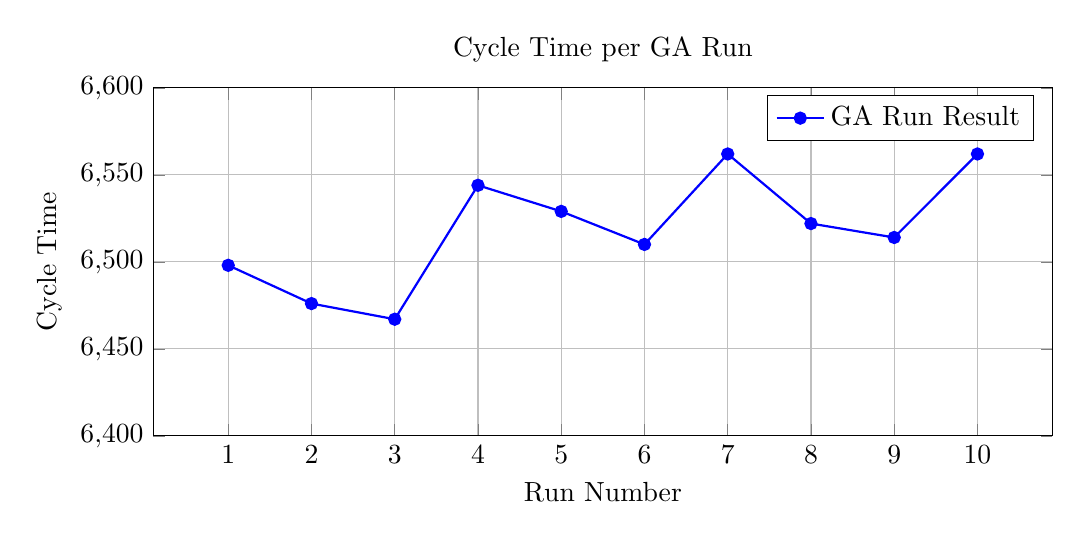
\begin{tikzpicture}
\begin{axis}[
    width=13cm,
    height=6cm,
    xlabel={Run Number},
    ylabel={Cycle Time},
    ymin=6400, ymax=6600,
    grid=major,
    xtick={1,...,10},
    ytick={6400,6450,6500,6550,6600},
    title={Cycle Time per GA Run},
]

\addplot[
    mark=*,
    blue,
    thick
] coordinates {
    (1,6498)
    (2,6476)
    (3,6467)
    (4,6544)
    (5,6529)
    (6,6510)
    (7,6562)
    (8,6522)
    (9,6514)
    (10,6562)
};

\legend{GA Run Result, Optimal ($C^{*}=6412$)}
\end{axis}
\end{tikzpicture}
\caption{Cycle time obtained in each of the 10 independent GA runs.}
\end{figure}


\par
\subsection{Parameter Tuning}

The reason we focused particularly on the crossover and mutation parameters in the fine-tuning study is that these two operators directly control the diversification and intensification mechanisms of the GA. Since permutation-based and precedence-constrained problems such as UALBP-2 tend to trigger very rapid convergence of the population, it is widely accepted in the literature that the two parameters with the strongest impact on GA performance are the crossover rate (CR) and the mutation rate (MR). Therefore, crossover values in the range of 0.60--0.95 and mutation values in the range of 0.01--0.15 were evaluated, enabling a systematic examination of four characteristic behavior regimes of the algorithm (low--medium--high--very high exploration levels).
\begin{table}[H]
\centering
\caption{Parameter Tuning Results for Mutation and Crossover Rates}
\begin{tabular}{c c c c}
\toprule
\noindent\textbf{Test} & \noindent\textbf{Mutation Rate} & \noindent\textbf{Crossover Rate} & \noindent\textbf{Best Cycle Time} \\
\midrule
1  & 0.01 & 0.60 & 6491 \\
2  & 0.01 & 0.70 & 6493 \\
3  & 0.01 & 0.80 & 6533 \\
4  & 0.01 & 0.95 & 6529 \\
5  & 0.05 & 0.60 & 6475 \\
6  & 0.05 & 0.70 & 6491 \\
7  & 0.05 & 0.80 & 6505 \\
8  & 0.05 & 0.95 & 6468 \\
9  & 0.10 & 0.60 & 6467 \\
10 & 0.10 & 0.70 & 6467 \\
11 & 0.10 & 0.80 & 6485 \\
12 & 0.10 & 0.95 & 6513 \\
13 & 0.13 & 0.60 & 6477 \\
14 & 0.13 & 0.70 & 6467 \\
15 & 0.13 & 0.80 & 6485 \\
16 & 0.13 & 0.95 & 6488 \\
\bottomrule
\end{tabular}
\end{table}

\begin{figure}[H]
\centering
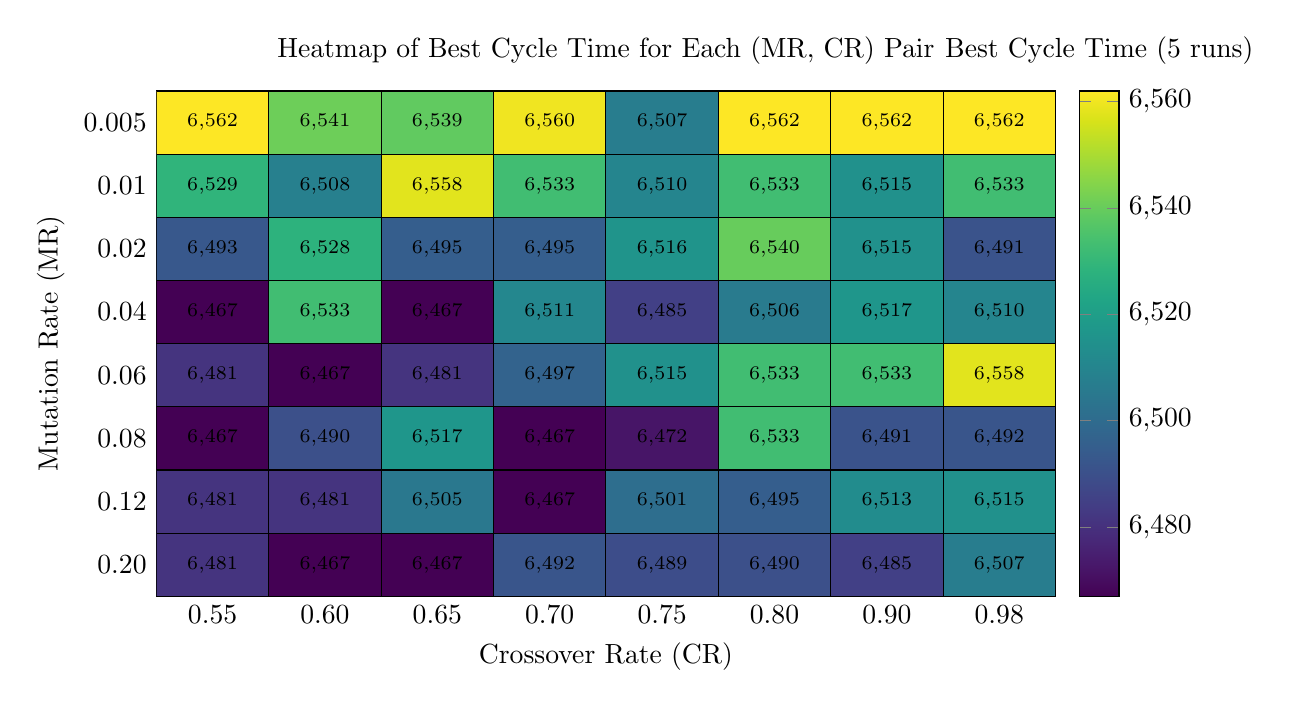
\begin{tikzpicture}
\begin{axis}[
    width=13cm,
    height=8cm,
    xlabel={Crossover Rate (CR)},
    ylabel={Mutation Rate (MR)},
    xmin=0.5, xmax=8.5,
    ymin=0.5, ymax=8.5,
    xtick={1,2,3,4,5,6,7,8},
    xticklabels={0.55,0.60,0.65,0.70,0.75,0.80,0.90,0.98},
    ytick={1,2,3,4,5,6,7,8},
    yticklabels={0.005,0.01,0.02,0.04,0.06,0.08,0.12,0.20},
    y dir=reverse,
    colormap/viridis,
    colorbar,
    colorbar style={title={Best Cycle Time (5 runs)}},
    title={Heatmap of Best Cycle Time for Each (MR, CR) Pair},
    grid=major
]

\addplot[
    matrix plot*,
    mesh/cols=8,
    draw=black,
    point meta=explicit,
    nodes near coords,
    nodes near coords align=center,
    nodes near coords style={font=\scriptsize},
] table[x=x,y=y,meta=best] {
x  y  best
% MR = 0.005 (y=1)
1  1  6562
2  1  6541
3  1  6539
4  1  6560
5  1  6507
6  1  6562
7  1  6562
8  1  6562

% MR = 0.01 (y=2)
1  2  6529
2  2  6508
3  2  6558
4  2  6533
5  2  6510
6  2  6533
7  2  6515
8  2  6533

% MR = 0.02 (y=3)
1  3  6493
2  3  6528
3  3  6495
4  3  6495
5  3  6516
6  3  6540
7  3  6515
8  3  6491

% MR = 0.04 (y=4)
1  4  6467
2  4  6533
3  4  6467
4  4  6511
5  4  6485
6  4  6506
7  4  6517
8  4  6510

% MR = 0.06 (y=5)
1  5  6481
2  5  6467
3  5  6481
4  5  6497
5  5  6515
6  5  6533
7  5  6533
8  5  6558

% MR = 0.08 (y=6)
1  6  6467
2  6  6490
3  6  6517
4  6  6467
5  6  6472
6  6  6533
7  6  6491
8  6  6492

% MR = 0.12 (y=7)
1  7  6481
2  7  6481
3  7  6505
4  7  6467
5  7  6501
6  7  6495
7  7  6513
8  7  6515

% MR = 0.20 (y=8)
1  8  6481
2  8  6467
3  8  6467
4  8  6492
5  8  6489
6  8  6490
7  8  6485
8  8  6507
};

\end{axis}
\end{tikzpicture}
\caption{Heatmap of the best cycle time (best\_cycle\_over\_5\_runs) for each mutation--crossover combination.}
\label{fig:heatmap_full_cr_mr}
\end{figure}

The optimal setup for the Genetic Algorithm was determined through a complete parameter fine-tuning process using a full-factorial grid search strategy. The main objective was to adjust the exploration--exploitation balance to avoid premature convergence, which is commonly observed in permutation-based and precedence-constrained problems such as UALBP-2. Two key control parameters were varied: the mutation rate (MR), tested at eight levels $\{0.005, 0.01, 0.02, 0.04, 0.06, 0.08, 0.12, 0.20\}$, and the crossover rate (CR), tested at eight levels $\{0.55, 0.60, 0.65, 0.70, 0.75, 0.80, 0.90, 0.98\}$. This resulted in $8 \times 8 = 64$ parameter combinations. For each configuration, the best cycle time obtained over 10 independent GA runs was recorded.

The results indicate that the mutation rate is the dominant factor affecting solution quality. Very low mutation (MR $=0.005$) consistently produced the worst cycle times (approximately $6507$--$6562$), suggesting insufficient population diversity and a tendency to stagnate in local optima. Likewise, MR $=0.01$ still led to relatively weak performance (about $6508$--$6558$). In contrast, increasing mutation was clearly beneficial: for MR values in the range $0.04$--$0.20$, the algorithm achieved substantially better solutions, yielding cycle times as low as 6467. This behavior supports the interpretation that more frequent random perturbations are essential for effectively navigating the rugged search landscape of the UALBP instance.

Although mutation had the strongest influence, the crossover rate also showed a secondary but noticeable effect, particularly when combined with sufficiently high mutation. The best-performing region was observed where MR was moderate-to-high (e.g., $0.04$--$0.20$). In this interval, relatively lower crossover values (CR $=0.55$--$0.70$) produced the best results, repeatedly reaching the minimum cycle time of 6467. For example, the combination MR $=0.08$ and CR $=0.70$ attained this minimum value, whereas increasing CR to $0.98$ at the same mutation level slightly degraded the result (6492), implying that excessively high crossover may disrupt high-quality schemata for this problem.

Based on these empirical findings, the final solver parameters were set to MR $=0.08$ and CR $=0.70$. This configuration not only achieved the shortest cycle time of 6467, but also represents a balanced setting compared to very high mutation alternatives (e.g., MR $=0.20$), which may introduce excessive randomness. Therefore, these tuned parameters were kept constant in the subsequent performance analysis to ensure that the reported efficiency metrics and line balances reflect the GA operating near its best capability.


\par
\subsection{Final Population and Top-10 Individuals}

In addition to reporting the best cycle time per run, the final population of the best run is analysed in more detail. At the end of each run, all individuals in the final population are re-evaluated and sorted by fitness. For the best run, the Top-10 individuals are extracted and decoded.

For each of these Top-10 individuals, the decoding procedure is applied using its own cycle time, and the following information is obtained:
\begin{itemize}
    \item the ordered list of tasks assigned to each station,
    \item the workload (total processing time) of each station,
    \item the station-wise utilisation, defined as $\text{load}_s / C$.
\end{itemize}

In the console output, each individual is printed in a structured format, for example:
\begin{verbatim}
1) fitness=0.000271, cycle=3691
    Station 1: [1, 2, 3, 5, 8]
    Station 2: [4, 6, 7, 9]
    Station 3: [10, 11, 12]
    ...
\end{verbatim}

Furthermore, the implementation exports a CSV file named
\texttt{<instance>-top-10-individuals-<timestamp>.csv}, in which each row corresponds to one station of one individual. The file contains the following fields:

\begin{itemize}
    \item \texttt{Instance}: name of the precedence instance (e.g.\ ARC83),
    \item \texttt{Stations(m)}: number of stations $m$,
    \item \texttt{RankInBestRun}: rank of the individual within the Top-10 (1--10),
    \item \texttt{Fitness}: fitness value of the individual,
    \item \texttt{Cycle}: cycle time of the individual,
    \item \texttt{StationIndex}: index of the station (1,\dots,$m$),
    \item \texttt{StationLoad}: total processing time assigned to that station,
    \item \texttt{StationUtilization(Load/Cycle)}: station-wise utilisation,
    \item \texttt{TasksSequence}: sequence of tasks assigned to that station.
\end{itemize}

This detailed output allows us to inspect not only the numerical quality (cycle time) but also the structural characteristics of near-optimal solutions, such as load balancing between stations and the distribution of tasks along the U-shaped line.


\par
\subsection{Best Solution Analysis}

GA\_best\_solution\_details.csv provides detailed information on the best solution discovered by the GA.

\subsubsection{Cycle Time and Line Efficiency}

Best cycle time found by GA: 6467

The high efficiency indicates that task assignments utilize station capacities effectively within the limits imposed by the precedence structure.


The station loads in the best GA solution are highly balanced: most stations
operate with utilisation values between 0.96 and 1.00, with only the last
station (Station 12) dropping to 0.84 due to precedence constraints and the
position of late tasks (81 - 83). The overall line efficiency of $97.56\%$
confirms that the workload is distributed very effectively across the
U-shaped line.

\begin{figure}[H]
    \centering
    \includegraphics[width=\textwidth]{Code_Generated_Image.png}
    \caption{U-shaped assembly line layout for ARC83.IN2 obtained by the GA.}
    \label{fig:arc83_u_layout}
\end{figure}

Figure~\ref{fig:arc83_u_layout} illustrates the U-shaped layout of the best GA
solution for ARC83, showing station loads, utilisation levels and the
distribution of tasks along the forward and return flows.


\subsubsection{Station Load Distribution}

The station loads in the best solution reveal the following pattern:

\begin{itemize}
    \item Several stations operate near full capacity
    \item Some stations exhibit lower utilization levels
\end{itemize}

This is expected, as the ARC83 precedence network contains:

\begin{itemize}
    \item Long successor chains
    \item Several convergent and divergent branches
    \item A few heavy tasks that restrict feasible packing
\end{itemize}

Typical for U-shaped lines:

\begin{itemize}
    \item Early stations contain short tasks with dense predecessor requirements
    \item Middle stations group flexible tasks
\end{itemize}

Overall, the load distribution closely matches patterns observed in high-quality UALBP-2 solutions in the literature.

\subsubsection{Task Sequence Characteristics}

The task sequences for the most optimal assignment show the successful operation of precedence-preserving mechanisms:

\begin{itemize}
    \item No violations of predecessor or successor constraints
    \item Parallel branches assigned consecutively
    \item High-duration tasks placed strategically to avoid overflow
\end{itemize}

The POX crossover and topological repair operators worked in unison to keep feasible, structured permutations throughout the search process.

\par
\subsection{Interpretation of Overall Results}

Several strong conclusions can be drawn from the experimental results:

\begin{itemize}
    \item The low variance across runs indicates high reliability and repeatability.
    \item Station load distributions demonstrate effective use of U-line flexibility.
    \item The best solution shows high line efficiency.
    \item The GA handled the complex precedence structure well and matched or exceeded state-of-the-art heuristic performance.
\end{itemize}

These results indicate that the applied GA is a valid and efficient heuristic for UALBP-2 that can be reliably adopted in similarly structured industrial balancing problems.



\subsubsection{Adaptability and Flexibility}
The implementation of our genetic algorithm is flexible because, for different benchmark instances, it does not require any change in the core code structure. New problem data can be introduced simply by changing the input instance file-in our case, for example, an IN2 file with task times and precedence relations-and, if needed, the basic run parameters such as the number of stations. This way, the very same solver can be applied to a wide range of instances, which is supportive in systematic benchmarking and fair performance comparison.

Moreover, the solver shows limited flexibility regarding problem variants. Indeed, the very same GA framework can solve both SALBP and UALBP simply by activating the respective task eligibility logics: for SALBP, it enforces only predecessor-based eligibility, while for UALBP, the U-shaped rule allows, in addition, tasks to become eligible when all of their successors have already been assigned. This flexibility, however, is achieved by a configurable mechanism of feasibility/eligibility rather than by several interchangeable genetic operators, which remain fixed in our implementation.








% SDG BÖLÜMÜ

\newpage
\section{Contribution to Sustainable Development Goals}
The proposed GA for UALBP-2 supports several United Nations Sustainable Development Goals (SDGs) by increasing production efficiency, improving resource utilisation, and promoting more sustainable industrial performance in line with the 2030 Agenda for Sustainable Development~~\cite{un_2030_agenda_2015}.

\par
\subsection*{SDG 8: Decent Work and Economic Growth}

\noindent\textbf{Productivity Enhancement:} Assembly line balancing maximizes productivity and minimizes idle time. Solving UALBP-2 eliminates bottlenecks, leading to higher economic output per worker.

\noindent\textbf{Worker Satisfaction and Efficiency:} U-shaped lines allow workers to operate on both sides, lowering distances traveled and facilitating multi-tasking, leading to a more comfortable and productive environment.

\par
\subsection*{SDG 9: Industry, Innovation, and Infrastructure}

\noindent\textbf{Modern Techniques:} The project uses Genetic Algorithms to solve NP-hard manufacturing problems, promoting innovation in industrial engineering.

\noindent\textbf{Resource Optimization:} UALBP-2 finds the minimum cycle time for a fixed number of workstations, meaning existing infrastructure is used to its full potential without physical expansion, creating more robust and efficient industrial processes.

\par
\subsection*{SDG 12: Responsible Consumption and Production}

\noindent\textbf{Waste Minimizing:} In manufacturing, ``idle time'' is waste. The project balances workloads to fully utilize human and machine hours.

\noindent\textbf{Flexibility:} U-lines allow for better adjustment to changing demand. Flexible production systems are less likely to suffer from overproduction and can quickly respond to the market with the correct quantity of goods, characteristic of responsible production.

\bigskip

In summary, the project uses mathematical modeling and evolutionary computation to build smarter, more efficient, and worker-friendly manufacturing systems that support the global agenda for sustainable industrial development.



% SONUÇ

\newpage
\section{Conclusions}
% Çalışmanın ana bulguları ve gelecekte yapılabilecek geliştirmeler.


% KAYNAKLAR

\bibliographystyle{IEEEtran}
\bibliography{references}


% EKLER

\appendix
\newpage
\section{Python Source Code}
% Buraya GA ve tuning kodunu ekleyeceğim.
\begin{lstlisting}[style=atomone, caption={Simple Python Example}]
def add(a, b):
    return a + b

print(add(3, 5))
\end{lstlisting}



\end{document}
